% chktex-file 44
%%%%%%%%%%%%%%%%%%%%%%%%%%%% ELC %%%%%%%%%%%%%%%%%%%%

\chapter{The Eclipsing Light Curve Code}\label{cha:ELC}

Having obtained the light curve of \groj, we attempted to model the data through numerical simulations of the X--ray binary. Here we outline the components of the model, and discuss the values obtained for the mass ratio and inclination.

%%%%%%%%%%%%%%%%%%%%%%%%%%%%% Introduction to ELC %%%%%%%%%%%%%%%%%%%%

\section{Introduction to \textit{ELC}}\label{cha:ELC:sec:IntroductionELC}

The \textbf{Eclipsing Light Curve} (\textit{ELC}) code%
\footnote{\label{cha:ELC:sec:IntroductionELC:foot:ELC}
We ran version 2 of this program, as described by the author in %
\citeN{OroszHauschildt:2000:cantcheck}%
}%
\ was written by Jerome A.\ Orosz, of the Universiteit Utrecht in
the Netherlands\footnote{\label{cha:ELC:sec:IntroductionELC:foot:Orosz}%
The author is now in San Diego State University. %
}%
. This suite of programs creates a theoretical model of a star
system, based on a user-specified set of parameters, such as the mass
ratio and orbital inclination of a binary system. It then modifies the
light curve until it obtains the best fit to the observations of the
user. %

\vspace{\myparskip}

The \textit{ELC} programs can model the light curve of:
\begin{itemize}


\item
\textbf{a binary star system}: for example, an X--ray binary, where the
companion star is denoted by star 1 and the compact star by star 2. %

\item
\textbf{a binary system with an accretion disk}, such as an X--ray binary with
a disk around the compact object (star 2). %

\end{itemize}
The component stars can have eccentric orbits, and the effect of
mutual eclipses of the accretion disk and secondary star can be
included in the model. %

\vspace{\myparskip}

The three \textit{ELC} programs that were employed in our modelling were:

\begin{itemize}

\item \texttt{ELC}%
\footnote{\label{cha:ELC:sec:IntroductionELC:foot:ELCabbrev}
Note that the abbreviation ELC can refer to either the suite of
programs (referred to in this text by the use of italics:
\textit{ELC}) or this specific program (referred to by using typewriter
font: \texttt{ELC}). }%
, which creates light curve models (in linear units) for several passbands
based on a list of system parameters. %

\item \mbox{\texttt{gridELC}}, an optimizer based on the ``grid search''
routine \cite{Bevington:1969}. Given a series of folded light curves and radial velocity curves,
\mbox{\texttt{gridELC}} will adjust user-specified parameters to find the
minimum $\Chi^2$ of the fit of the \textit{ELC} model to the data. The
final set of parameters are then used to create light curve models
(in linear units).

\item \mbox{\texttt{checkfit}}, which converts the linear
\texttt{gridELC} model to magnitudes and then scales it according to the
data. %

\end{itemize}

We utilised these \textit{ELC} programs to model both the 1998 and
1995 data sets. %

%%%%%%%%%%%%%%%%%%%%%%%%%%%%% 1998 $K_s$--band Data %%%%%%%%%%%%%%%%%%%%

\section{The 1998 $K_s$--band Data}\label{cha:ELC:sec:1998Results}

%%%%%%%%%%%%%%%%%%%%%%%%%%%%% Details of Model %%%%%%%%%%%%%%%%%%%%

\subsection{Details of the Quiescent Model}\label{cha:ELC:sec:1998Results:subsec:model}

The quiescent observations of \groj\ were modelled by accounting only
for the ellipsoidal variability of the secondary star. The disk contribution to
the overall flux of the system was assumed to be negligible (we will later show this to
be a valid assumption -- see \S~%
\vref{cha:AccretionDiskContamination:sec:Spectroscopy:subsec:DiskContribution}%
), and hence we assumed there would be no noticeable eclipse of the
accretion disk. It was also assumed that there was no X--ray heating of
the secondary star. The model we employed was of a binary system
with a Roche lobe filling secondary star and a black hole primary
star. %

%%%%%%%%%%%%%%%%%%%%%%%%%%%%% Modelling Procedure %%%%%%%%%%%%%%%%%%%%

\subsection{Modelling Procedure for the 1998 Data}\label{cha:ELC:sec:1998Results:subsec:ModellingProcedure}

The following procedure details how we modelled the 1998 observations
of \\%
% WHITE SPACE %
\groj\ using the described model. %

\begin{itemize}

\item
We obtained a folded light curve for the 1998 $K_s$--band observations
(see \S~%
\vref{cha:lightcurve:sec:Photometry:subsec:RelativePhotometry}%
). This light curve was phased according to the convention of %
\citeN{OroszBailyn:1997}%
\ which places star 1 (with filled Roche lobe) in front of the compact star 2 at phase 0.0. See
Figure~%
\vref{cha:lightcurve:sec:Photometry:subsec:RelativePhotometry:fig:kctio98plot}%
\ for the plot of this light curve. %

\begin{table}[htb]
\caption{Fixed \textit{ELC} Binary System Parameters}\label{cha:ELC:sec:1998Results:subsec:ModellingProcedure:tab:FixELCBinaryParms}

\begin{minipage}{\linewidth}
\renewcommand{\thefootnote}{\thempfootnote}


\DeclareFixedFootnote{\beerstellar}{Corresponding to a star of spectral type
F5--G0 III--IV (Beer \& Podsiadlowski 2001).} % For fixed footnote
\DeclareFixedFootnote{\pringle}{This close binary should have synchronously rotating components in a circular orbit.} % For fixed footnote %(Pringle 1985)
\DeclareFixedFootnote{\ob97}{Orosz \& Bailyn (1997).} % For fixed footnote
\DeclareFixedFootnote{\vdh98}{van~der~Hooft et~al.\ (1998).} % For fixed footnote
\DeclareFixedFootnote{\shah}{Shahbaz et~al.\ (1999).} % For fixed footnote
\DeclareFixedFootnote{\beer}{Beer \& Podsiadlowski (2001) -- these values were only initially fixed.} % For fixed footnote
\DeclareFixedFootnote{\bh}{\textit{ELC} interprets this to mean that the primary star is an invisible black hole.} % For fixed footnote

\begin{center}
\begin{tabular}{|l||||l|c|}

\hline
Name        & Description                & Value \\\hline\hline\hline\hline
Q        & Mass ratio                 & 3.9\beer \\\hline
finc        & Inclination                 & $68\fdg65$\beer \\\hline
Tgrav1      & Gravity Darkening exponent, star 1    & 0.25\vdh98 \\\hline
Period        & Orbital period of binary            & 2 \fd 62168\vdh98 \\\hline
betarim        & Angle of disk to orbital plane     & $\sim 2\degr$\ob97  \\\hline
alb1        & Bolometric albedo, star 1        & 0.5\ob97\\\hline
fm        & Mass function, star 2            & 2.73\,M\ensuremath{_{\odot}}\shah \\\hline
separ        & Orbital separation            & $\sim16$\,R\ensuremath{_{\odot}}\shah \\\hline
Teff1        & Mean temperature, star 1        & $\sim6400$\,K\beerstellar \\\hline
Teff2        & Mean temperature, star 2        & $<0$\,K\bh \\\hline
fill1        & Roche lobe filling factor, star 1     & 1.000%
\footnote{\label{cha:ELC:sec:1998Results:subsec:ModellingProcedure:tab:FixELCBinaryParms:foot:mass}%
Since accretion continues in quiescence (see \S~\vref{cha:Introduction:sec:X--rayBinaries:subsec:Quiescence}). }%
\\\hline
fill2        & Roche lobe filling factor, star 2    & 0.000%
\footnote{\label{cha:ELC:sec:1998Results:subsec:ModellingProcedure:tab:FixELCBinaryParms:foot:bh}
Primary star is a black hole.}%
\\\hline
eccen        & Eccentricity of orbit            & 0\pringle \\\hline
omega1        & Ratio of rotational to orbital frequency, star 1 & 1\pringle \\\hline
omega2        & Ratio of rotational to orbital frequency, star 2 & 1\pringle \\\hline

\hline

\end{tabular}
\end{center}
\end{minipage}
\end{table}

\nocite{OroszBailyn:1997}
\nocite{Shahbaz_et_al.:1999}
%\nocite{Pringle:1985}
\nocite{BeerPodsiadlowski:2001}

\begin{table}[htb]
\caption{Fixed \textit{ELC} Parameters}\label{cha:ELC:sec:1998Results:subsec:ModellingProcedure:tab:FixELCParms}

\begin{minipage}{\linewidth}
\renewcommand{\thefootnote}{\thempfootnote}

\begin{center}
\begin{tabular}{|l||||l|c|}

\hline
Name        & Description                & Value \\\hline\hline\hline\hline
Nalph1, Nalph2     & Number of latitude grid elements     & 100 \\\hline
Nbet1, Nbet2    & Number of longitude grid elements     & 35  \\\hline
Ntheta        & Number of azimuthal grid points    & 90 \\\hline
Nradius        & Number of radial grid points        & 80 \\\hline
ilaw        & Controls form of limb darkening law    & 1 (Linear
law)  \\\hline

\hline

\end{tabular}
\end{center}
\end{minipage}
\end{table}

\item
The literature was consulted for values of the parameters in Table~%
\vref{cha:ELC:sec:1998Results:subsec:ModellingProcedure:tab:FixELCBinaryParms}%
. The values for the parameters in Table~%
\vref{cha:ELC:sec:1998Results:subsec:ModellingProcedure:tab:FixELCParms} %
were set from experience. %

\begin{table}[htb]
\caption{Values of Variable \textit{ELC} Parameters for 1998 Data}\label{cha:ELC:sec:1998Results:subsec:ModellingProcedure:tab:VarELCParms}

\begin{minipage}{\linewidth}
\renewcommand{\thefootnote}{\thempfootnote}
\DeclareFixedFootnote{\nodisk}{No disk present.} % For fixed footnote
\DeclareFixedFootnote{\nolx}{No X--ray heating.} % For fixed footnote
\DeclareFixedFootnote{\noeclipse}{No eclipses.} % For fixed footnote

\begin{center}
\begin{tabular}{|l||||l|c|}

\hline
Name        & Description &    Value \\\hline\hline\hline\hline
iecheck & Switch for eclipses & -1\noeclipse  \\\hline
idint & Switch for disk       & 0\nodisk \\\hline
rinner        & Inner radius of disk  & --\nodisk \\\hline
router        & Outer radius of disk    & --\nodisk \\\hline
xi        & Power-law exponent on the disk temperature profile &
--\nodisk \\\hline
tdisk        & Temperature of inner disk & --\nodisk \\\hline
Nref        & Number of iterations for reflection effect & 0\nolx \\\hline
Lx        & $\log_{10}{L_{X}}$ for primary star in X--ray binary
& 0\nolx \\\hline

\hline

\end{tabular}
\end{center}
\end{minipage}
\end{table}

\item
Since this model ignored X--ray heating and the accretion disk, the
parameters in Table~%
\vref{cha:ELC:sec:1998Results:subsec:ModellingProcedure:tab:VarELCParms} %
were set to the appropriate values. %

\item
\texttt{ELC} was run without a input file to produce a
\textbf{parameter file} with each parameter
set to its default value. This file was edited, setting the parameters
to the values shown in Tables~%
\ref{cha:ELC:sec:1998Results:subsec:ModellingProcedure:tab:FixELCBinaryParms}%
--%
\ref{cha:ELC:sec:1998Results:subsec:ModellingProcedure:tab:VarELCParms}. %
The remaining parameters were left at their default values.

\item
\texttt{ELC} was run once more, this time using the \textbf{edited}
input file. This created a model binary system based on the values
given for the system parameters, and outputted this in both
linear and magnitude units to a data file. %

\item
The parameter file for \mbox{\texttt{gridELC}} was edited, to specify
both the folded light curve data file and the parameters to be adjusted, namely the
mass ratio and inclination. %

\item
\mbox{\texttt{gridELC}} was run. The final values calculated for the adjusted
parameters were noted.

\item
The $\Chi^2$ value of the fit of the model to the observations was
determined using \mbox{\texttt{checkfit}}, from which the reduced
chi-squared%
\footnote{\label{cha:ELC:sec:IntroductionELC:foot:chi2}
%(\citeN{McCarthy:1999} p.~19) %
The reduced chi-squared ($\Chi^{2}_{\nu}$) of the fit is defined by: %
\[ \Chi^{2}_{\nu} = \frac{\Chi^2}{n-p-1}, \]
where $n$ is the number of the data points and $p$ is the number of
parameters of the fit. A $\Chi^{2}_{\nu}$ value of approximately 1 was
desired. }%
\ was calculated. %

\item The resultant model plot and the light curve data were
superimposed for a visual check of the fit. %
\end{itemize}%

%%%%%%%%%%%%%%%%%%%%%%%%%%%%% Comparison of Model and Results %%%%%%%%%%%%%%%%%%%%

\subsection{Comparison of Quiescent Model and Results}\label{cha:ELC:sec:1998Results:subsec:comparison}%

%%%%%%%%%%%%%%%%%%%%%%%%%%%%% kctio98fit %%%%%%%%%%%%%%%%%%%%
\begin{figure}[!htb]%
\begin{center}%
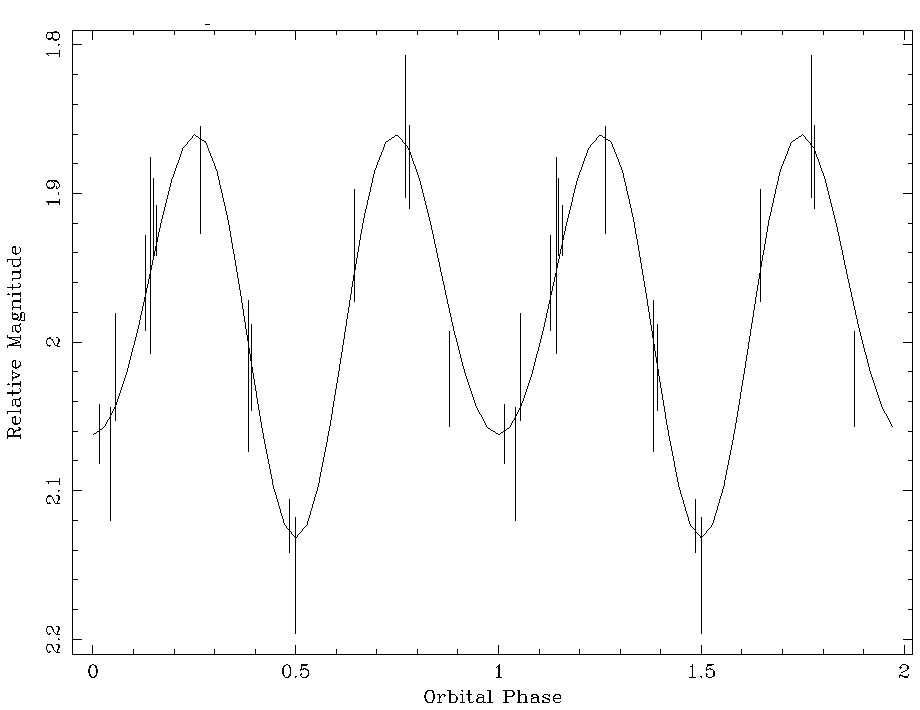
\includegraphics[width=5.0in]{kctio98fit}%
\caption{%
The observed $K_s$ light curve for \groj\ in May/June 1998, together with a theoretical light curve computed for a mass ratio of $2$ and a binary inclination of $69\degr$. %
Two orbital cycles are shown for clarity.}\label{cha:ELC:sec:1998Results:subsec:comparison:fig:kctio98fit}%
\end{center}%
\end{figure}%
%%%%%%%%%%%%%%%%%%%%%%%%%%%%%%%%%%%%%%%%%%%%%%%%%%%%%%%%%%%%%%%%%%

As can be seen in Figure~%
\vref{cha:ELC:sec:1998Results:subsec:comparison:fig:kctio98fit}%
, the data were well modelled by our theoretical light curve, and we
obtained $\Chi_{\nu}^{2} = 0.51$ as the reduced chi-squared%
\footnote{\label{cha:ELC:sec:1998Results:foot:LowError}
We interpret this low $\Chi_{\nu}^{2}$ value as signifying that
\texttt{DAOPHOT} is overestimating the errors for the estimates of the
relative magnitude of \groj. }. %
The theoretical light curve mimics the ellipsoidal variability of the
secondary, with the expected deeper minimum at phase 0.5. %

%%%%%%%%%%%%%%%%%%%%%%%%%%%%% Derived Mass Ratio and Inclination %%%%%%%%%%%%%%%%%%%%

\subsubsection{Derived Mass Ratio and Inclination}\label{cha:ELC:sec:1998Results:subsec:comparison:subsubsec:derivedQ}

%%%%%%%%%%%%%%%%%%%%%%%%%%%%% contourPlot2  %%%%%%%%%%%%%%%%%%%%
\begin{figure}[!htb]
\begin{center}
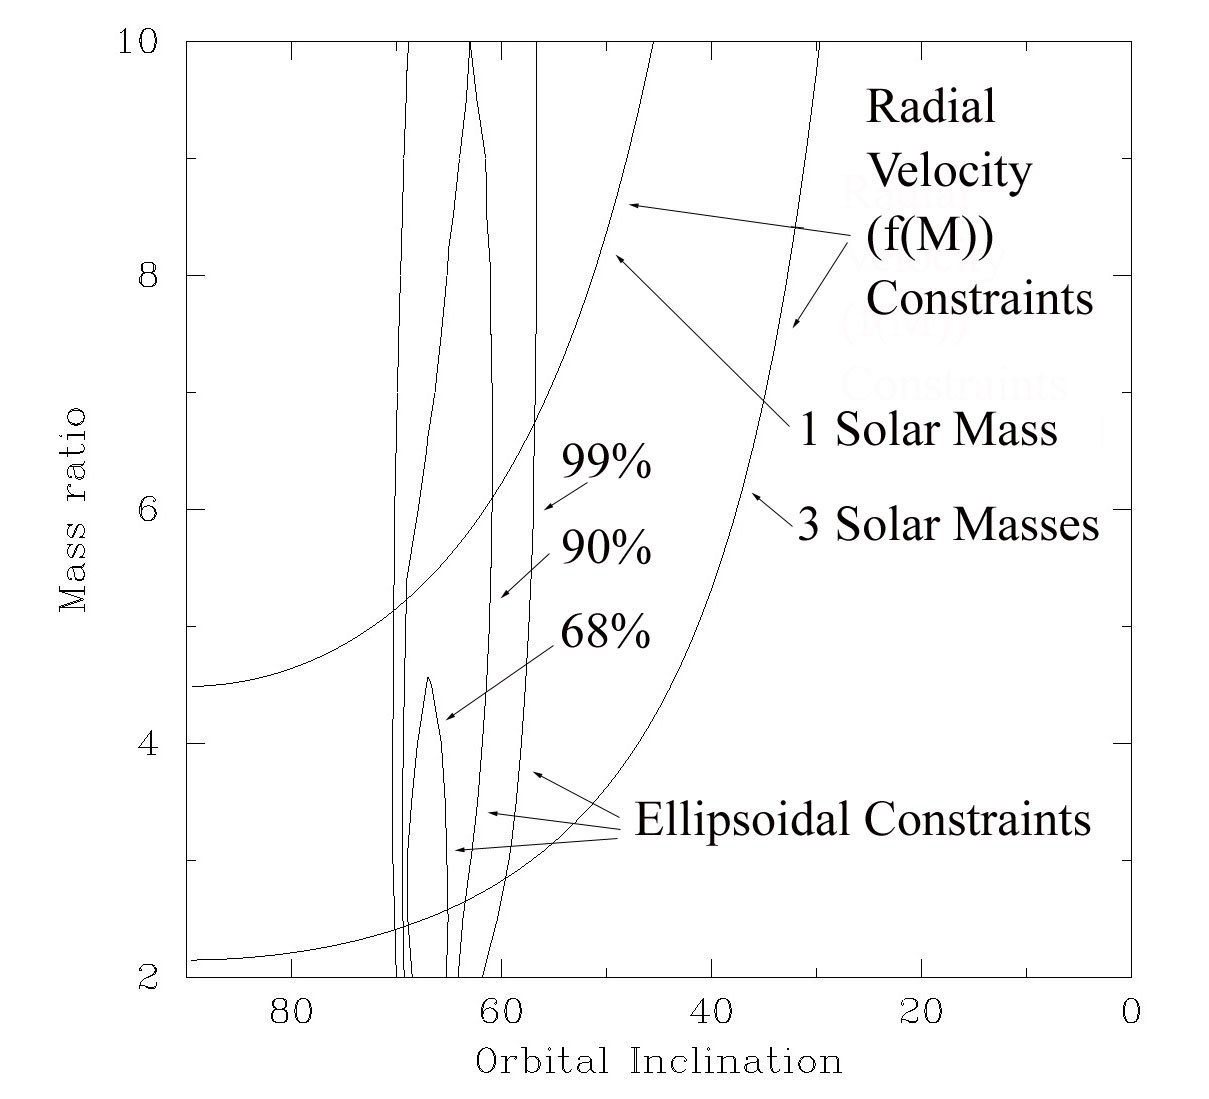
\includegraphics[width=5.0in]{contourPlot2}
\caption{%
The $\chi^2$ contour plot for the 1998 $K_{s}$--band data. This plot displays the 68\%, 90\% and
 99\% confidence levels from the \texttt{ELC} fits, together with constraint curves derived from the mass function assuming a secondary mass of 1\,M\sun and 3\,M\sun, respectively. (The minimum reduced $\chi^2$ has been set equal to 1.) %
}\label{cha:ELC:sec:1995Results:subsec:comparison:fig:contourPlot2}
\end{center}
\end{figure}

%%%%%%%%%%%%%%%%%%%%%%%%%%%%%%%%%%%%%%%%%%%%%%%%%%%%%%%%%%%%%%%%%%

In order to properly constrain the mass ratio and the inclination, \texttt{gridELC} was run to create a $\Chi^{2}$ contour plot. We simultaneously varied the inclination between $i=0\degr$ and $i=90\degr$ and the mass ratio between $q=2$ and $q=10$, and computed the $\Chi^{2}$ of the fit using \texttt{gridELC}. Figure~%
\vref{cha:ELC:sec:1995Results:subsec:comparison:fig:contourPlot2}%
\ shows the resultant plot, together with constraints for $i$ and $q$
derived from the mass function and secondary mass considerations,
assuming (conservatively) that the mass of the secondary lies between 1\,M\sun and
3\,M\sun -- it is an F/G (sub)giant. The area in Figure~\ref{cha:ELC:sec:1995Results:subsec:comparison:fig:contourPlot2} where the mass function and ellipsoidal modelling constraints overlap denotes the allowed values of $q$ and $i$. Generally, our results show that the inclination of the system lies in the range $i=64\degr$--$70\degr$, and that the mass ratio lies in the range $q=2.5$--$6$, at the 90\% confidence level. %

\vspace{\myparskip}

Table~%
\vref{cha:ELC:sec:1998Results:tab:ComparisonOfResults}%
\ compares the values we derived for the mass ratio $q$ and the
inclination $i$ of \groj\ with those from other studies of this system. From this table, it can be seen that the values for both our mass ratio and orbital inclination are
consistent with past estimates. %

\begin{table}[htb]
\caption{Comparison of Derived Values for $q$ and $i$}\label{cha:ELC:sec:1998Results:tab:ComparisonOfResults}

\begin{minipage}{\linewidth}
\renewcommand{\thefootnote}{\thempfootnote}

\begin{center}
\begin{tabular}{|l||||c|c|}

\hline
Data Set            & $q$          & $i$ \\\hline\hline\hline\hline
Our 1998 $K_s$--band Data     & $2.5-6$     & $64\degr-70\degr$
\\\hline
\citeN{BeerPodsiadlowski:2001} (Predicted) & $3.9\pm0.6$    & $68\fdg65\pm1\fdg5$ \\\hline
\citeN{GreeneBailynOrosz:2001}    & $2.6\pm0.3$    & $70\fdg2\pm1\fdg9$ \\\hline
\citeN{Shahbaz_et_al.:1999}    & 2.29--2.97 & -- \\\hline
van~der~Hooft et~al.\ \citeyear{VanDerHooft_et_al.:1998}    & 2.43--4.20     & $63\fdg7$--$70\fdg7$\\\hline
\citeN{OroszBailyn:1997}    & $2.99\pm0.08$    & $69\fdg50\pm0\fdg08$ \\\hline

\hline

\end{tabular}
\end{center}
\end{minipage}
\end{table}


%%%%%%%%%%%%%%%%%%%%%%%%%%%%% Derived Component Masses %%%%%%%%%%%%%%%%%%%%

\subsubsection{Derived Component Masses}\label{cha:ELC:sec:1998Results:subsec:comparison:subsubsec:derivedm}

Using our values for $q$ from the 1998 data ($q=2.5$--$6$) and the
corresponding secondary masses ($M_{2}=1$--$3$\,M\sun), we derived the
mass of the primary as $6.8\pm0.7$\,M\sun. This is to be compared in particular with the results from the only other infrared study of this system, which yielded $M_{X}=6.3\pm0.5$\,M\sun \cite{GreeneBailynOrosz:2001}. Table~%
\vref{cha:ELC:sec:1998Results:subsec:comparison:subsubsec:derivedm:tab:ComparisonOfResults}%
\ compares this mass with masses from earlier studies. %

\begin{table}[htb]
\caption{Comparison of Derived Values for $M_X$}\label{cha:ELC:sec:1998Results:subsec:comparison:subsubsec:derivedm:tab:ComparisonOfResults}

\begin{minipage}{\linewidth}
\renewcommand{\thefootnote}{\thempfootnote}

\begin{center}
\begin{tabular}{|l||||c|c|}

\hline
Data Set            & $M_X$ (M\sun)      \\\hline\hline\hline\hline
Our 1998 $K_s$--band Data     & $6.8\pm0.7$        \\\hline % 2002Bin2SimpleMassInc
\citeN{BeerPodsiadlowski:2001} (Predicted) & $5.4\pm0.3$    \\\hline
\citeN{GreeneBailynOrosz:2001}    & $6.3\pm0.5$    \\\hline
\citeN{Shahbaz_et_al.:1999}    & 5.5--7.9 \\\hline
van~der~Hooft et~al. \citeyear{VanDerHooft_et_al.:1998}    & 6.29--7.20     \\\hline
\citeN{OroszBailyn:1997}    & $7.02\pm0.22$    \\\hline

\hline

\end{tabular}
\end{center}
\end{minipage}
\end{table}

\vspace{\myparskip}

Our values are consistent with preceding results, and is above the
standard limit for neutron star masses. This implies that the compact
object in \groj\ is a black hole, if we accept the neutron star mass limit of \citeN{RhoadesRuffini:1974}. We note however that this result is dependent on the assumption of negligible disk contamination. %

%%%%%%%%%%%%%%%%%%%%%%%%%%%%% 1995 $K_s$--band Data %%%%%%%%%%%%%%%%%%%%

\section{The 1995 $K_s$--band Data}\label{cha:ELC:sec:1995Results}

%%%%%%%%%%%%%%%%%%%%%%%%%%%%% Details of Model %%%%%%%%%%%%%%%%%%%%

\subsection{Details of Outburst Model}\label{cha:ELC:sec:1995Results:subsec:model}

The model for the outburst of \groj\ included:
\begin{inparaenum}[(i)]
\item
the ellipsoidal variability of the Roche lobe filling secondary,
\item
a bright hot accretion disk and
\item
eclipses of the accretion disk and the secondary.
\end{inparaenum}

%%%%%%%%%%%%%%%%%%%%%%%%%%%%% Modelling Procedure %%%%%%%%%%%%%%%%%%%%

\subsection{Modelling Procedure for the 1995 Data}\label{cha:ELC:sec:1995Results:subsec:ModellingProcedure}

\begin{table}[htb]
\caption{Values of Variable \textit{ELC} Parameters for 1995 Data Set}\label{cha:ELC:sec:1995Results:subsec:ModellingProcedure:tab:paramvalues}

\begin{minipage}{\linewidth}
\renewcommand{\thefootnote}{\thempfootnote}

\DeclareFixedFootnote{\steady}{Assuming a steady-state disk.} % For fixed footnote
\DeclareFixedFootnote{\diskp}{Accretion disk present.} % For fixed footnote
\DeclareFixedFootnote{\eclipse}{Check for eclipses.} % For fixed footnote
\DeclareFixedFootnote{\nolx}{No X--ray heating.} % For fixed footnote

\begin{center}
\begin{tabular}{|l||||l|}

\hline
Name        & Value \\\hline\hline\hline\hline
iecheck     & 0\eclipse\\\hline
idint         & 1\diskp \\\hline
rinner        & 0.55   \\\hline
router        & 1.0      \\\hline
xi        & $-0.8$\steady \\\hline
tdisk        & $\sim 13000$\,K \\\hline
Nref        & 0\nolx \\\hline
Lx        & 0\nolx \\\hline

\hline

\end{tabular}
\end{center}
\end{minipage}
\end{table}

The procedure for modelling the 1995 $K_s$ observations was
essentially the same as for the 1998 data. Here, we outline the main
differences:

\begin{itemize}

\item
The variable parameters were set as to include an accretion disk and
eclipses -- see Table~%
\vref{cha:ELC:sec:1995Results:subsec:ModellingProcedure:tab:paramvalues}%
. %

\item
Rather than attempting to vary the mass ratio and inclination, we
fixed these parameters to the values obtained from the quiescent data,
and applied these values in our attempt to fit the outburst data.

\end{itemize}

%%%%%%%%%%%%%%%%%%%%%%%%%%%%% Comparison of Model and Results %%%%%%%%%%%%%%%%%%%%

\subsection{A Poor Fit}\label{cha:ELC:sec:1995Results:subsec:comparison}

%%%%%%%%%%%%%%%%%%%%%%%%%%%%% kctio95fixedfit %%%%%%%%%%%%%%%%%%%%
\begin{figure}[!htb]
\begin{center}
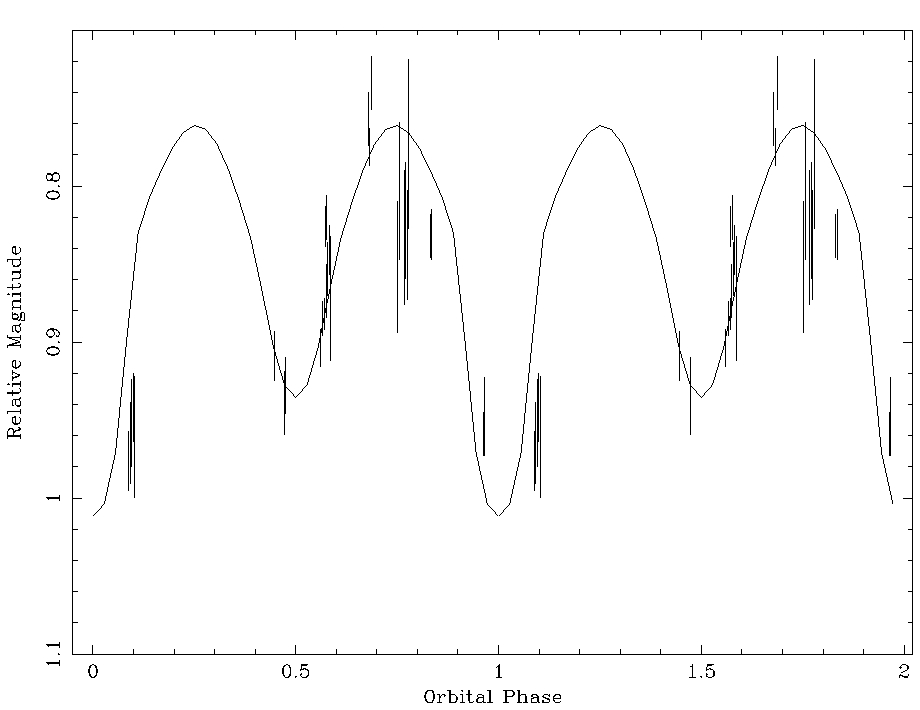
\includegraphics[width=5.0in]{kctio95fixedfit}
\caption{%
The June 1995 $K_s$ light curve of \groj, with a model
light curve using the mass ratio and inclination from the best fits of
the 1998 data set ($q=2$, $i=69\degr$). %
}\label{cha:ELC:sec:1995Results:subsec:comparison:fig:kctio95fixedfit}
\end{center}
\end{figure}
%%%%%%%%%%%%%%%%%%%%%%%%%%%%%%%%%%%%%%%%%%%%%%%%%%%%%%%%%%%%%%%%%%

Figure~%
\vref{cha:ELC:sec:1995Results:subsec:comparison:fig:kctio95fixedfit}%
\ shows the resultant fit of our model to the outburst data. We
obtained a reduced chi-squared of $\Chi_{\nu}^{2} = 5.89$. The fit is much poorer than for the 1998 data, for the reasons we now outline. %

%%%%%%%%%%%%%%%%%%%%%%%%%%%%% The Accretion Disk %%%%%%%%%%%%%%%%%%%%

\subsubsection{The Accretion Disk}\label{cha:ELC:sec:1995Results:subsec:comparison:subsubsec:disk}

Since \groj\ was in outburst at the time of these observations, the
flux from the accretion disk was more significant than the ellipsoidal
variability of the secondary star. The deeper minimum at phase 0 is
indicative of an eclipse of the bright accretion disk by the
secondary star. The presence of eclipses agrees well with the high
orbital inclination of this system. %

\vspace{\myparskip}

We note that there is no evidence of an eclipse of the accretion disk
in the quiescent light curve, even though \groj\ has been shown to be
an eclipsing binary from the outburst observations, and in spite of the high inclination ($i\sim70\degr$) of the system. This is consistent
with the negligible disk contribution to the overall flux from the
system during quiescence. %

\vspace{\myparskip}

The reduced $\Chi^2$ values obtained for the outburst data are
significantly higher than the quiescent values. One possible
explanation for this is that the accretion disk is significantly
non-axisymmetric, or exhibits infrared flaring or flickering activity, which the code is unable to account for. %
\citeN{OroszBailyn:1997}%
\ were also unable to accurately model their optical outburst data, taken
during August 1994 and March--April 1995, and obtained larger reduced
$\Chi^2$ values from modelling their outburst data than from their quiescent data. %

%%%%%%%%%%%%%%%%%%%%%%%%%%%%% Amplitude of Variability %%%%%%%%%%%%%%%%%%%%

%%%%%%%%%%%%%%%%%%%%%%%%%%%% Confirming Our Assumption of Negligible Disk Contribution
 %%%%%%%%%%%%%%%%%%%%

\section{Does the Accretion Disk Contribute?}\label{cha:ELC:sec:ConfirmingOurAssumption}

Although we have now obtained a plausible value for the mass of the black hole in \groj, we made the assumption that the contribution of the accretion disk in the infrared was negligible. In the following chapter, we explain how we confirmed this assumption from infrared spectroscopy of the binary system.

%%%%%%%%%%%%%%%%%%%%%%%%%%%%% End of Chapter %%%%%%%%%%%%%%%%%%%%
